\section{Model definition}
\label{model-definition}

This Section gives an overview of the models used on the different 
training sets. We first start with the multilayer perceptrons and 
end with the convolutional networks used on the image dataset.

For both models we present the architecture, the initial results 
and the hyperparameter tuning phase.

\subsection{Multilayer perceptron}

The first model used in the experiments is a Multilayer perceptron. 
The considered training sets are the ones presented on Subsection 2.2 and 2.3 minus the image 
dataset, 
namely the first and extended datasets. For the first one, scaled and unscaled 
versions are considered, while for the second the normal and PCA version are tested.

\subsubsection{Network structure}
The starting point for the neural network structure is a 
reasonable network in terms of hidden neurons to prevent over-fitting, 
indeed a high number of units in the hidden layers would end up in learning 
too much from the dataset, leading to poor performances on the test sets.

For this reason, the rule of thumb followed to decide hidden neurons quantity is the 
following: 
$$\#\mathit{hidden\; neurons} = \frac{2}{3}\big(\#\mathit{input\;neurons}
+ \#\mathit{output\;neurons}\big)$$
The next step is to decide the hidden layers number. As using the rule 
presented above gives a quite small amount of units, only two layers are considered,  
indeed, an higher quantity would mean having a real small number of neurons per layer.

Applying this rule ended up in the following architectures on the four 
different training sets, where the output layer is fixed at 10:
\begin{center}
    \begin{tabular}{ |l|r|r|r| } 
        \hline
        Training set & Input & 1st Hidden & 2nd Hidden  \\
        \hline
        132 features unscaled &  132 & 60 & 30 \\
        132 features scaled &  132 & 60 & 30 \\
        180 features scaled &  180 & 80 & 46 \\
        102 features reduced with PCA &  102 & 45 & 30 \\
        \hline
    \end{tabular}
\end{center}

To build the actual model \emph{Tensorflow} and \emph{Keras} libraries 
are used.~\cite{tensorflow}\cite{keras}

\paragraph{Starting point model}
To give reference, Figure \ref{mod} shows the model used on the PCA training set, mentioned at 
the end of Subsection \vref{extended-dataset}, with 
102 input features.
\begin{figure}
    \begin{center}
        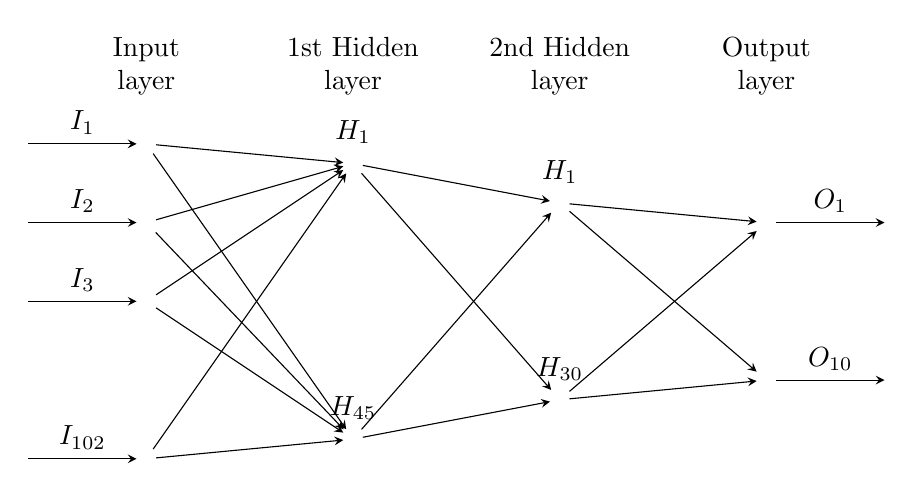
\begin{tikzpicture}[x=1.5cm, y=1cm, >=stealth]
            
            % layers
            \foreach \m/\l [count=\y] in {1,2,3,missing,4}
            \node [every neuron/.try, neuron \m/.try] (input-\m) at (0,2.5-\y) {};
            
            \foreach \m [count=\y] in {1,missing,2}
            \node [every neuron/.try, neuron \m/.try ] (hidden-\m) at (1.75,3-\y*1.75) {};
            
            \foreach \m [count=\y] in {1,missing,2}
            \node [every neuron/.try, neuron \m/.try ] (hidden2-\m) at (3.5,2-\y*1.25) {};
            
            \foreach \m [count=\y] in {1,missing,2}
            \node [every neuron/.try, neuron \m/.try ] (output-\m) at (5.25,1.5-\y) {};
            
            %   label
            \foreach \l [count=\i] in {1,2,3,{102}}
            \draw [<-] (input-\i) -- ++(-1,0)
            node [above, midway] {$I_{\l}$};
            
            \foreach \l [count=\i] in {1,45}
            \node [above] at (hidden-\i.north) {$H_{\l}$};
            
            \foreach \l [count=\i] in {1,30}
            \node [above] at (hidden2-\i.north) {$H_{\l}$};
            
            \foreach \l [count=\i] in {1,10}
            \draw [->] (output-\i) -- ++(1,0)
            node [above, midway] {$O_{\l}$};
            
            \foreach \i in {1,...,4}
            \foreach \j in {1,...,2}
            \draw [->] (input-\i) -- (hidden-\j);
            
            \foreach \i in {1,...,2}
            \foreach \j in {1,...,2}
            \draw [->] (hidden-\i) -- (hidden2-\j);
            
            \foreach \i in {1,...,2}
            \foreach \j in {1,...,2}
            \draw [->] (hidden2-\i) -- (output-\j);
            
            \foreach \l [count=\x from 0] in {Input, 1st Hidden, 2nd Hidden, Output}
            \node [align=center, above] at (\x*1.75,2) {\l \\ layer};
        \end{tikzpicture}
    \end{center}
    \caption{Multilayer perceptron architecure used on the PCA dataset}
    \label{mod}
\end{figure}

This last model, with the one built to predict the 180 features training set, are the ones selected for 
the hyperparameter tuning phase. 

\paragraph{Activation and loss functions}
The activation function for the input and hidden layers is a \emph{Relu}, 
typically used to prevent the \emph{vanishing gradient problem}, 
and the output one uses a \emph{Softmax} to have classification probabilities
among classes.~\cite{relu}\cite{soft}\cite{vanishing}\\
The loss used is the \emph{Sparse Categorical Crossentropy loss} as it 
is well suited for multiclass classification and, since 
the classes are integers and not one-hot encoded, the sparse version is preferred.~\cite{entropy}

\paragraph{Choosing an optimizer}
When choosing an optimizer for a neural network one must take into account the 
cost of reaching a minimum point on the error function.
Although more complex optimizers exist, build to reduce training 
cost or achieve better performances on deep networks, the one choosen 
for this model is a classic Stochastic Gradient Descent optimizer.

\subsubsection{Training set results}

Section \vref{feature-extraction} talks about the four different 
training sets obtained from the dataset and, without going into details, 
states that there is continuous improvement. 
We now give a more detailed look on training performances, after 
detailing how class imbalance is faced and the applied validation method.

Note that all the random seeds used by Tensorflow are fixed 
to make results reproducible. This step is necessary as many parameters initial 
value is random, for instance, the neural network weights.

\paragraph{Class imbalance}
To deal with the minority of some classes, balancing techniques should be 
applied when fitting the model. One of the possible approaches, and the one followed
here, is to assign class weights. 

The main idea is to penalize errors made on not well represented classes to account 
for their minority, in particular, each class has weight:
$$w_i = \frac{\#\mathit{total\;samples}}{\#\mathit{classes} * \#\mathit{samples\;of\;class\;i}}$$
Class weights computation relies on the \emph{compute class weights} function with the balanced logic
from sklearn.~\cite{classweight}\\
The following are the computed quantities for the dataset classes:
\begin{center}
    \begin{tabular}{ |l|c|c| } 
        \hline
        Class name & Number of samples & Class weight \\
        \hline
        air conditioner & 500 & 0.8998 \\
        car horn & 208 & 2.1629 \\
        children playing & 500 & 0.8998 \\
        dog bark & 500 & 0.8998 \\
        drilling & 500 & 0.8998 \\
        engine idling & 517 & 0.8702 \\
        gun shot & 190 & 2.3678 \\
        jackhammer & 548 & 0.8209 \\
        siren & 536 & 0.8393 \\
        street music & 500 & 0.8998 \\
        \hline
    \end{tabular}
\end{center}
As expected, the less numerous classes have higher class weight than the rest,
in particular, the misclassification of a car horn sample
counts more than double than an air conditioner one.

\paragraph{Stratified cross-validation}
To estimate performance on the training set, stratified cross-validation with 
five folds is used. Basically the dataset is divided into five parts 
and a model is repeatedly trained on four and tested on one, all while considering class 
distribution, indeed, the original distribution of the classes is maintained 
in the splits.~\cite{stratified}

The stratified approach is required as there is class imbalance on the training set.
In fact, applying a classical cross-validation could show misleading results, 
for instance when the minority classes are more present 
in the test fold rather than the training ones; in such cases the loss would be 
higher.
The mean accuracy on the test folds gives a hint about the model performance.

For this step the \emph{Stratified KFold} class from scikit learn is used.~\cite{cross-scikit}

\paragraph{Results}
The following are the results on the training sets, using the architectures 
presented at the beginning of the Subsection.
\begin{center}
    \begin{tabular}{ |l|r|r| } 
        \hline
        Training set & Mean accuracy & St. deviation \\
        \hline
        132 features unscaled &  0.1138 & 0.0039 \\
        132 features scaled &  0.5743 & 0.0324 \\
        180 features scaled &  0.6363 & 0.0494 \\
        102 features reduced with PCA &  0.6188 & 0.0420 \\
        \hline
    \end{tabular}
\end{center}

There is a great improvement after scaling the training set, after 
that small refinements are made.
As accuracy is the best on the last two training sets, those are the two selected to 
perform the hyperparameter tuning.

\subsubsection{Hyperparameter tuning}

The last two tries with feature extraction lead to the best results 
with stratified cross-validation. Although the two models are reasonable, 
they can not be the final ones as many parameters are left on their default value, 
for instance, learning rate and momentum of the optimizer are untouched. 

The main goal now is to experiments with ranges of model parameters 
to find a better one. From now on, the model build on the 180 features training set is 
called \emph{Extended model}, 
while the one tested on the PCA training set is named \emph{PCA model}.

\paragraph{Grid and random search comparison}
Two of the most commonly used strategies in hyperparameter optimization
are \emph{grid} and \emph{random search}~\cite{random-grid}. 

In both cases we define ranges of parameters to test different combinations, 
for instance, fixed the number of neurons, one could try to find the best 
combination of learning rate and momentum that optimize accuracy on the training set.

While similar, the two methodologies differs in the amount of exploration they do.
The grid search try all the possible combinations of parameters, while the 
random approach fixes a number of iterations and picks an arbitrary unseen 
combination each time. 

Obviously the first one is more computationally expensive than the second, if 
we fix a small amount of possible iterations, but in theory it finds a better result
than going the random route. 
Nonetheless the grid search can led to over-fitting and in practice random 
search in preferred.

\paragraph{Random search}
We now run a random search with various parameters 
to optimize the initial models.
Note that class weights are still considered and the models are evaluated
again with a stratified cross-validation.
The optimizer used is the stochastic gradient descent.

The considered ranges for parameters for this run are: 
\begin{enumerate}
    \item \emph{Neurons}: input layer has dimension $I$ and last layer $O$, while 
    the two hidden layers are tested with a number of neurons respectively 
    equals to: 
    $$H_1 + 2i\;\;\text{and}\;\;H_2 + 2j,\;\;\text{with}\;\; i, j \in \{-2,-1,0,1,2\}$$
    \item \emph{Learning rate}: $0.001, 0.01, 0.1, 0.5$;
    \item \emph{Momentum}: $0.0, 0.01, 0.1, 1$;
    \item \emph{Epochs}: $60, 80, 100$;
    \item \emph{Batch size}: $32, 64$.
\end{enumerate}

Where $I$, $H_1$, $H_2$ and $O$ are input, first hidden, second hidden 
and output layer dimensions, thus they depend on the initial architecture.
As stated before, the two models considered are the following: 
\begin{center}
    \begin{tabular}{ |l|r|r|r|r|} 
        \hline
        Model name & $I$ & $H_1$ & $H_2$ & $O$ \\
        \hline
        Extended model & 180 & 80 & 46 & 10 \\
        PCA model & 102 & 45 & 30 & 10 \\
        \hline
    \end{tabular}
\end{center}

An \emph{early stopper} with patience equals to three is used on the training to stop it when no progress is made with 
respect to the last three epochs result.~\cite{early}
The search is performed with 100 iterations for both rounds.

\paragraph{Final models}
The first round of the random search, performed on the Extended model, resulted 
in the following parameters:
\begin{itemize}
    \item Neurons: 180 for input, 76 for the first hidden layer, 50 for the second and 10 for output;
    \item Momentum: 0.01
    \item Learning rate: 0.01
    \item Epochs: 80
    \item Batch size: 64
\end{itemize}
We can see an improvement in accuracy by comparing it to the starting point model:
\begin{center}
    \begin{tabular}{ |l|r|r| } 
        \hline
        Model & Mean accuracy & St. deviation \\
        \hline
        Initial extended model & 0.6363 & 0.0494\\
        Tuned extended model & 0.6497 & 0.0431\\
        \hline
    \end{tabular}
\end{center}

The second random search on the smaller PCA model, resulted in this results:
\begin{itemize}
    \item Neurons: 102 for input, 45 for the first hidden layer, 32 for the second and 10 for output;
    \item Momentum: 0.01
    \item Learning rate: 0.1
    \item Epochs: 80
    \item Batch size: 32
\end{itemize}
As before, comparing it with the starting model, we can see some better results:
\begin{center}
    \begin{tabular}{ |l|r|r| } 
        \hline
        Model & Mean accuracy & St. deviation \\
        \hline
        Initial PCA model & 0.6188 & 0.0420\\
        Tuned PCA model & 0.6270 & 0.0315\\
        \hline
    \end{tabular}
\end{center}

\subsection{Convolutional neural network}
This subsection presents the results obtained by a convolutional
neural network trained on the image datasets presented at the end of 
Section \vref*{feature-extraction}.
We start by giving an overview of the network, to then proceed 
with the training results and hyperparameter tuning.

\subsubsection{Network structure}
The structure of a neural network for image classification 
consists of convolutional layers followed by pooling layers, 
and, at the end, densely connected ones to have the output classification.

The main idea is to extract relevant features from the images 
with the convolutional layers, that apply a kernel to the input 
to detect patterns and image features.
After the convolution part there is a pooling layer that reduces dimensionality.

Taking inspiration from the \emph{VGG19 architecture}, that stacks two or more 
convolutional layers to then apply pooling, the network is built with 
the following layers:~\cite{vgg}
\begin{itemize}
    \item \emph{Convolution}: 16 filters, kernel size of $3 \times 3$, Relu activation
    \item \emph{Convolution}: 16 filters, kernel size of $3 \times 3$, Relu activation
    \item \emph{MaxPooling}: pooling size of $2 \times 2$, 2 strides
    \item \emph{Convolution}: 32 filters, kernel size of $3 \times 3$, Relu activation
    \item \emph{Convolution}: 32 filters, kernel size of $3 \times 3$, Relu activation
    \item \emph{MaxPooling}: pooling size of $2 \times 2$, 2 strides
    \item \emph{Flatten}
    \item \emph{Dense}: 100 neurons and Relu activation
    \item \emph{Dense}: 40 neurons and Relu activation
    \item \emph{Output}: 10 neurons and softmax activation
\end{itemize}

\subsubsection{Training set results}
To have an idea of the performances of the initial convolutional network,
a cross validation is performed on the image training set. 

As before, a stratified cross-validation is used with five folds, thus, 
results can be compared to the multilayer perceptrons previously trained.
\begin{center}
    \begin{tabular}{ |l|r|r| } 
        \hline
        Training set & Mean accuracy & St. deviation \\
        \hline
        Tuned extended model& 0.6497 & 0.0431 \\
        Tuned PCA model & 0.6270 & 0.0315 \\
        Image dataset & xxx &  xxx \\
        \hline
    \end{tabular}
\end{center}

\subsubsection{Hyperparameter tuning}
Training a CNN is really expensive compared to the multilayer perceptrons.
Performing a full random search is infeasible with the resources we have, therefore, 
to have an idea about the impact on accuracy of the network parameters, 
we run cross validation on the following models:
\begin{itemize}
    \item x
    \item x
    \item x
    \item x
\end{itemize}

\paragraph{Final training results}
\begin{center}
    \begin{tabular}{ |l|r|r| } 
        \hline
        Training set & Mean accuracy & St. deviation \\
        \hline
        Tuned extended model& 0.6497 & 0.0431 \\
        Tuned PCA model & 0.6270 & 0.0315 \\
        Image dataset & xxx &  xxx \\
        \hline
    \end{tabular}
\end{center}

\newpage